\chapter{Symmetry, Energy, and the Hamiltonian}

After a long informal prelude, Leonard Susskind returns to what he calls half the heart of the subject: symmetry and conservation laws. The lecture is corrective in tone before it becomes constructive. We first repair the meaning of symmetry itself, especially the distinction between active and passive transformations; only then do we return to Noether charges, ask the missing question about energy, and derive the Hamiltonian. These notes follow Leonard Susskind's Lecture~5 in that order, and the preserved board figures are kept here as lecture evidence, with visual curation for note writing by LazyingArt LLC and Video2Book.

\section{Returning to Symmetry}

Susskind begins by saying that his previous discussion of symmetry was not sufficiently clear. The point of repair is not a minor notational matter. It is the physical meaning of the transformation itself.

Take a particle on a line and the instruction
\[
x \to x+1.
\]
What does this mean? There are two different operations hiding inside the same symbols.

The passive version merely relabels the points on the line. A point that used to carry the label \(x=0\) is now called \(x'=1\), but nothing in the physical system has moved. If the particle sits in a potential, the potential energy does not change, because the particle has not changed its position relative to the world.

The active version keeps the labels fixed and moves the particle. If the particle was at \(x\), we take it to \(x+1\). Now the potential energy may change, because the particle has moved relative to the environment that created the potential in the first place.

That last phrase matters. A particle moving in a potential is already a split description of a larger system. The particle is the part we track; the Earth, or the apparatus, or some other heavy external structure is treated as fixed. If we moved the entire universe, including the Earth and the source of the potential, then the potential energy would not change. But that is not the approximation we are making. We are studying motion relative to a fixed external structure, and for this reason the active transformation is the right one to keep in mind.

Once this is clear, the lecture passes from \(x\) to generalized coordinates \(q_i\). Configuration space is the space of all \(q_i\), and a configuration of the system is a point in that space. An active infinitesimal transformation moves every point of configuration space by a prescribed little amount,
\begin{equation}
\delta q_i=\epsilon f_i(q),
\end{equation}
where \(\epsilon\) is a small bookkeeping parameter and the functions \(f_i(q)\) may depend on position in configuration space. The shift is fixed once and for all, but it need not be the same at different points.

The lecture also imposes an important restriction: the functions \(f_i\) are taken to be independent of time. Under that assumption the change in the velocity is obtained by differentiating the change in the coordinate:
\begin{equation}
\delta \dot q_i=\frac{d}{dt}\,\delta q_i.
\end{equation}
For a pure translation \(x\to x+\epsilon\), the shift is constant, so
\begin{equation}
\delta \dot x=0.
\end{equation}
But for a coordinate-dependent transformation, such as a rotation, the velocity does change, precisely because the coordinate change itself depends on the coordinates.

\section{When Is a Transformation Really a Symmetry?}

An active transformation will generally change the potential energy. It may even change the kinetic energy. In Cartesian coordinates the kinetic energy often looks simple, but in more general coordinates it can depend on the coordinates themselves. Polar coordinates already teach the lesson:
\[
T \sim r^2 \dot\theta^2.
\]
So under a general infinitesimal transformation there is no reason for either \(T\) or \(V\) to remain fixed separately.

What, then, is a symmetry? Susskind insists on two points.

First, it is the whole Lagrangian that matters. Second, the condition must hold everywhere in configuration space, not merely at the particular point where the system happens to sit along its actual motion.

A simple example captures both statements. Suppose the potential energy is \(V(x,y)\), and suppose we make an infinitesimal shift in the \(x\)-direction. Then the first-order change in \(V\) is
\begin{equation}
\delta V=\frac{\partial V}{\partial x}\,\delta x.
\end{equation}
If this vanishes for every possible position of the system, then
\begin{equation}
\frac{\partial V}{\partial x}=0,
\end{equation}
so the potential is independent of \(x\). If the same statement held for shifts in every direction, the potential would be constant. This is the meaning of saying that the potential does not change under the transformation.

The Lagrangian criterion is the same in spirit: under an infinitesimal symmetry, there is no first-order change in \(L\). It is convenient to write this schematically as
\begin{equation}
\delta L = O(\epsilon^2),
\end{equation}
with the understanding that the lecture states this verbally rather than as a formal theorem. One does not worry about the \(O(\epsilon^2)\) terms; if the first-order change vanishes everywhere, then repeated infinitesimal steps build a finite transformation that also leaves the Lagrangian unchanged.

We also make the standard smoothness assumption. The lecture briefly pauses over worries about cusps and nonunique derivatives, then sets them aside. The discussion concerns differentiable functions, so that first-order variations make sense.

\subsection{Question \& Answer}

\paragraph{Question.} Must the kinetic and potential energies each remain invariant separately? And when we say that the Lagrangian does not change, do we mean exactly zero or merely a tiny change?

\paragraph{Answer.} No separate invariance of \(T\) and \(V\) is required. In many cases the Lagrangian does not split neatly into kinetic and potential pieces at all; it is simply a function of \(q\) and \(\dot q\). The symmetry condition is a condition on the whole Lagrangian. And because the transformation is infinitesimal, the natural statement is that there is no change to first order in the small parameter. That is the real content of ``no change.''

\section{Noether Charge: Translation and Rotation}

Once the criterion for symmetry has been sharpened, Susskind returns to the conserved quantity. If
\[
\delta q_i=\epsilon f_i(q)
\]
is an ordinary symmetry, then the conserved Noether charge is
\begin{equation}
Q=\sum_i p_i f_i(q),
\qquad
p_i=\frac{\partial L}{\partial \dot q_i},
\qquad
\dot Q=0.
\end{equation}
In the lecture he remarks that he had previously called the conserved quantity \(q\) for ``quantity.'' Here we use the more transparent notation \(Q\).

The simplest example is translation. If we shift only \(x\), then \(f_x=1\), and the corresponding conserved quantity is just the momentum \(p_x\). If the system is fully translation invariant in three-dimensional space, then \(p_x\), \(p_y\), and \(p_z\) are all conserved. If there are many particles, the symmetry is the simultaneous displacement of all of them, and the conserved quantity is the total momentum.

Rotation is the next example, and it is slightly richer. In the plane, an infinitesimal rigid rotation takes the form
\begin{equation}
\delta x=-y\,\epsilon,
\qquad
\delta y=x\,\epsilon.
\end{equation}
To check that this really is a rotation, we may test the squared distance from the origin:
\begin{equation}
r^2=x^2+y^2.
\end{equation}
Its variation is
\begin{equation}
\delta(r^2)=2x\,\delta x+2y\,\delta y.
\end{equation}
Substituting the rotational shifts,
\[
\delta(r^2)=2x(-y\epsilon)+2y(x\epsilon)=0,
\]
so the transformation preserves distance from the origin, as a rigid rotation should.

Because the coordinates change, the velocities change as well:
\begin{equation}
\delta \dot x=-\dot y\,\epsilon,
\qquad
\delta \dot y=\dot x\,\epsilon.
\end{equation}
This is exactly what one expects from the rule \(\delta \dot q_i = d(\delta q_i)/dt\). The kinetic energy in the combination \(\dot x^2+\dot y^2\) is therefore unchanged by the rotation, and if the potential depends only on the radial distance, the entire Lagrangian is invariant.

The conserved quantity follows mechanically from the Noether formula:
\begin{equation}
Q=p_x(-y)+p_y(x)=-y\,p_x+x\,p_y.
\end{equation}
This is the \(z\)-component of angular momentum,
\begin{equation}
Q=(\mathbf r\times \mathbf p)_z.
\end{equation}
In three dimensions one gets all three components by rotating about the three coordinate axes, and for many-particle systems one sums the angular momenta of all particles:
\[
\mathbf L_{\mathrm{tot}}=\sum_a \mathbf r_a\times \mathbf p_a.
\]

The lecture emphasizes again that translation and rotation symmetry refer to the whole system. If we hold some massive external object fixed and study motion relative to it, the symmetry may be lost because the potential energy changes.

\section{Time Translation and the Hamiltonian}

Having repaired ordinary symmetries, Susskind comes to the missing conservation law.

\subsection{Question \& Answer}

\paragraph{Question.} Is energy conservation also associated with a symmetry?

\paragraph{Answer.} Yes. But it is not an ordinary shift in the coordinates \(q_i\). The relevant symmetry is translation in time.

The lecture introduces time translation invariance experimentally. Imagine an experiment beginning at time \(t_0\), ending at time \(t_1\), and producing some outcome. Now shift the whole experiment later by an amount \(\delta t\): start later, end later, keep the initial conditions otherwise the same, and ask whether the outcome changes. If it does not, then the system is time-translation invariant.

There are obvious ways for this symmetry to fail if we isolate only part of a larger system. A charged particle between capacitor plates provides one example. If the field between the plates is being ramped up externally, then the outcome depends on when we start the experiment. A harmonic oscillator with a time-dependent spring constant provides another:
\begin{equation}
L=\frac12 m\dot x^2-\frac12 k(t)x^2.
\end{equation}
If \(k\) varies with time, then knowing \(x\) and \(\dot x\) is not enough to know the value of \(L\); one must also know the time. This is what explicit time dependence means.

Susskind compresses the criterion to a sentence: time translation invariance means no explicit time dependence in the Lagrangian. In formulas, we may write
\begin{equation}
\frac{\partial L}{\partial t}=0.
\end{equation}
This does not mean that \(L\) is numerically constant along the motion. The coordinates and velocities still change with time. It means only that \(L\) has no additional dependence on \(t\) beyond that inherited from \(q(t)\) and \(\dot q(t)\).

He then begins the derivation of the Hamiltonian in a deliberately playful way. Suppose, he says, one guessed that the Lagrangian itself might be the conserved energy. There is an easy test: compute \(dL/dt\) and see whether it vanishes.

\begin{figure}[htbp]
\centering

\includegraphics[width=0.62\textwidth]{lecture_05_figure_02.png}
\caption{Beginning the calculation of the time derivative of the Lagrangian.}
\end{figure}

Starting from the total derivative along the trajectory,
\begin{equation}
\frac{d}{dt}L(q_i,\dot q_i),
\end{equation}
the chain rule gives
\begin{equation}
\frac{dL}{dt}
=
\sum_i \frac{\partial L}{\partial q_i}\dot q_i
+
\sum_i \frac{\partial L}{\partial \dot q_i}\ddot q_i
+
\frac{\partial L}{\partial t}.
\end{equation}
Now we use two familiar ingredients:
\begin{equation}
p_i=\frac{\partial L}{\partial \dot q_i},
\qquad
\dot p_i=\frac{\partial L}{\partial q_i}.
\end{equation}
Substituting them,
\begin{equation}
\frac{dL}{dt}
=
\sum_i \left(\dot p_i\dot q_i+p_i\ddot q_i\right)
+
\frac{\partial L}{\partial t}.
\end{equation}
The bracketed sum is a product rule:
\begin{equation}
\sum_i \left(\dot p_i\dot q_i+p_i\ddot q_i\right)
=
\frac{d}{dt}\sum_i p_i\dot q_i.
\end{equation}
Therefore
\begin{equation}
\frac{d}{dt}\left(L-\sum_i p_i\dot q_i\right)
=
\frac{\partial L}{\partial t}.
\end{equation}
This identifies the conserved combination. We define the Hamiltonian by
\begin{equation}
H=\sum_i p_i\dot q_i-L,
\end{equation}
and so obtain the central relation
\begin{equation}
\frac{dH}{dt}=-\frac{\partial L}{\partial t}.
\end{equation}
When there is no explicit time dependence, \(\partial L/\partial t=0\), and therefore \(\dot H=0\).

\begin{figure}[htbp]
\centering

\includegraphics[width=0.55\textwidth]{lecture_05_figure_04.png}
\caption{The clean board statement of the Hamiltonian time-dependence relation.}
\end{figure}

For the familiar one-particle Lagrangian
\[
L=\frac12 m\dot x^2-V(x),
\]
we have \(p=m\dot x\), and so
\begin{equation}
H=p\dot x-L
=
m\dot x^2-\left(\frac12 m\dot x^2-V(x)\right)
=
\frac12 m\dot x^2+V(x).
\end{equation}
Thus in the ordinary separable case the Hamiltonian is simply the total energy \(T+V\).

The time-dependent oscillator shows how the general formula works when energy is not conserved. For
\[
L=\frac12 m\dot x^2-\frac12 k(t)x^2,
\]
we hold \(x\) and \(\dot x\) fixed and differentiate only the explicit time dependence:
\begin{equation}
\frac{\partial L}{\partial t}
=
-\frac12 \dot k(t)x^2.
\end{equation}
Hence
\begin{equation}
\dot H=\frac12 \dot k(t)x^2.
\end{equation}
The oscillator exchanges energy with the external agent that changes the spring constant. From the narrower point of view, energy is not conserved. From the broader point of view, where the agent is included, the full energy is conserved.

\section{Board Recap and the Usefulness of Lagrangian Mechanics}

At this stage the lecture pauses and gathers the formalism into a compact board summary.

\begin{figure}[htbp]
\centering

\includegraphics[width=0.58\textwidth]{lecture_05_figure_03.png}
\caption{A compact recap: the general Lagrangian, canonical momentum, and the start of the Euler--Lagrange equation.}
\end{figure}

The recap is conceptually useful because it shows what now belongs to the toolkit:
\begin{align}
L &= L(q_i,\dot q_i,t), \\
p_i &= \frac{\partial L}{\partial \dot q_i}, \\
\dot p_i &= \frac{\partial L}{\partial q_i}, \\
Q &= \sum_i p_i f_i(q), \qquad \dot Q=0, \\
\dot H &= -\frac{\partial L}{\partial t}.
\end{align}
The board handwriting makes \(p_i\) look like a capital \(P\), but the mathematics is the ordinary canonical momentum.

This is also where the lecture turns from foundations to usefulness. Why should one bother with the Lagrangian when Newton's laws often suffice? Susskind's answer is pragmatic: the Lagrangian is a powerful way to organize a problem when the choice of variables matters.

The double pendulum is his example. The brute-force Newtonian description is possible, but awkward. One must keep track of constraint forces at the pivot and at the joint, and one rapidly drowns in components. The Lagrangian method begins differently: choose coordinates that fit the geometry, compute the kinetic and potential energies in those coordinates, subtract them, and only then derive the equations of motion.

\begin{figure}[htbp]
\centering

\includegraphics[width=0.82\textwidth]{lecture_05_figure_05.png}
\caption{The Hamiltonian relation remains on the board while the double-pendulum example is introduced.}
\end{figure}

A clean schematic version of the sketch is worth keeping near the screenshot:

\begin{figure}[htbp]
\centering
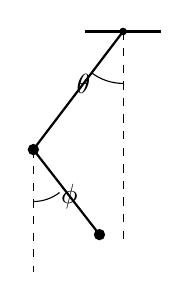
\begin{tikzpicture}[scale=1.2]
\draw[thick] (-0.4,0) -- (0.4,0);
\fill (0,0) circle (0.04);
\draw[dashed] (0,0) -- (0,-2.2);
\draw[thick] (0,0) -- (-0.95,-1.25);
\fill (-0.95,-1.25) circle (0.06);
\draw[dashed] (-0.95,-1.25) -- (-0.95,-2.55);
\draw[thick] (-0.95,-1.25) -- (-0.25,-2.15);
\fill (-0.25,-2.15) circle (0.06);
\draw (0,-0.55) arc (-90:-127:0.55);
\node at (-0.42,-0.55) {$\theta$};
\draw (-0.95,-1.8) arc (-90:-52:0.45);
\node at (-0.57,-1.75) {$\phi$};
\end{tikzpicture}
\caption{A cleaned schematic of the double pendulum suggested by the board sketch.}
\end{figure}

The lecture does not work out the full equations here, but the method is clear. Choose angular coordinates, express the velocities of the masses in terms of \(\theta\), \(\phi\), \(\dot\theta\), and \(\dot\phi\), form \(T-V\), and then apply the Euler--Lagrange equations. This is much easier than trying to transform a large set of Newtonian force equations by hand.

The same practical lesson applies to change of variables more generally. If one wants rotating coordinates, for example, it is usually simpler to transform the Lagrangian than to transform the equations of motion term by term.

Susskind also pauses here to compare the Lagrangian and Hamiltonian viewpoints. They are equivalent, but they emphasize different features. The Lagrangian emphasizes stationary action; the Hamiltonian is more abstract, but it will later become central in quantum mechanics.

\section{A Nonstandard Lagrangian and the Limits of the Formalism}

The lecture closes the main mathematical discussion with a deliberately nonstandard example. The point is not that one should start from this particular model, but that the formalism itself does not require the most familiar \(T-V\) form in order to make sense.

Take
\begin{equation}
L=\frac12 q^2\dot q^2-\frac12 q^2.
\end{equation}
Susskind remarks in passing that one could add other mixed terms such as \(q\dot q\), but the worked example is the one written above.

The momentum conjugate to \(q\) is
\begin{equation}
p=\frac{\partial L}{\partial \dot q}=q^2\dot q.
\end{equation}
Its time derivative is
\begin{equation}
\dot p=q^2\ddot q+2q\dot q^2.
\end{equation}
On the other hand,
\begin{equation}
\frac{\partial L}{\partial q}=q\dot q^2-q.
\end{equation}
Thus the Euler--Lagrange equation becomes
\begin{equation}
q^2\ddot q+2q\dot q^2=q\dot q^2-q,
\end{equation}
or, after simplification,
\begin{equation}
q^2\ddot q+q\dot q^2=-q.
\end{equation}

\begin{figure}[htbp]
\centering

\includegraphics[width=0.78\textwidth]{lecture_05_figure_06.png}
\caption{The intermediate algebraic step in the nonstandard example.}
\end{figure}

The Hamiltonian is computed in the same way as always:
\begin{equation}
H=p\dot q-L.
\end{equation}
Since \(p=q^2\dot q\),
\begin{equation}
H=q^2\dot q^2-\left(\frac12 q^2\dot q^2-\frac12 q^2\right)
=
\frac12 q^2\dot q^2+\frac12 q^2.
\end{equation}
In this particular example the result again looks like a sum of two positive terms, and one may choose to call them \(T\) and \(V\). But the lecture's point is broader: the Hamiltonian provides the general definition of energy even when the split into conventional kinetic and potential terms is not especially natural.

From here the lecture turns to the boundaries of the formalism. What about friction? Susskind's answer is emphatic: ordinary finite-degree-of-freedom Lagrangian mechanics does not directly describe friction. Friction is a collective, statistical effect of very many microscopic degrees of freedom that we do not keep track of. The same remark applies to inelastic collisions. One may model the center-of-mass motion approximately, but once heat, internal excitations, and hidden microscopic motions matter, the simple few-coordinate description is no longer the whole story.

The lecture then asks a larger question. Why does classical mechanics have this Lagrangian and Hamiltonian form at all? One answer is empirical: real systems behave that way. One answer is heuristic: we may guess a Lagrangian from symmetry or reverse-engineer it from equations of motion. But Susskind insists that the deeper explanation points beyond classical mechanics itself. Quantum mechanics is logically prior. One can write mathematically consistent equations, such as simple first-order laws like \(\dot x=-x\), but they are not the sort of fundamental mechanical systems realized in nature. The deeper reason is postponed, but the direction is clear: the abstract calculus of classical mechanics is tied to quantum mechanics.

\section{Summary}

This lecture does three things in sequence. It clarifies symmetry by insisting on the active viewpoint and on invariance of the whole Lagrangian, everywhere in configuration space, to first order in the infinitesimal parameter. It then uses this sharpened idea to recall Noether charges for translation and rotation. Finally, it asks the missing question about energy, answers it through time translation invariance, and derives the Hamiltonian as
\[
H=\sum_i p_i\dot q_i-L.
\]

The remaining discussion widens the perspective. The Lagrangian method is not merely a formal restatement of Newtonian mechanics; it is often the natural way to set up a problem, especially when the right coordinates are not Cartesian. And although the Hamiltonian reduces to \(T+V\) in familiar cases, its significance is broader than that special form. The lecture ends by pointing outward: friction belongs to many hidden degrees of freedom, and the deeper reason this whole calculus works as it does lies, ultimately, in quantum mechanics.